
\subsection{Sensor data}

The sensors send the data to the mobile application over BLE. The protocol as well as the hardware architecture of the devices places restrictions on the sample width and sampling rate. BLE protocol specifies maximum \SI{80}{\byte} per message, and minimum duration of \SI{7.5}{\milli\second} between messages; this gives us theoretical maximum of \SI{10640}{\byte\per\second}. With one particular hardware / firmware implementation, we found that the effective reliable data transfer rate drops to only \SI{280}{\byte\per\second}. That particular device also lacked significant processing power. This gave us baseline protocol for 3-axis samples (such as acceleration or rotation), with \SI{20}{\byte} for header and \SI{5}{\byte} per sample. Packing the sample values into \SI{40}{\bit} gave us $3 \times$\SI{13}{\bit} and \SI{1}{\bit} for padding, and yielded code in \autoref{lst:threed-data}.

\begin{lstlisting}[language=C,caption={BLE 3-axis data},label={lst:threed-data}]
#define PACKED __attribute__((__packed__))

struct PACKED threed_data {
    int16_t x_val : 13;           // 13
    int16_t y_val : 13;           // 26
    int16_t z_val : 13;           // 39
    int16_t _     : 1;            // 40
};

struct PACKED header {
    uint16_t preamble;            // 2
    uint8_t type_count;           // 3
    uint8_t samples_per_second;   // 4
    uint32_t timestamp;           // 12
    uint32_t sample_count;        // 16
    uint32_t type;                // 20
};
\end{lstlisting}

The \lstinline{preamble} is a marker sequence, which also allows for detection of endian-ness; though all sensor data-collecting devices we have encountered so far are big endian. The payload consisting of \lstinline{header} followed by 50 samples of \lstinline{threed_data} results in \SI{270}{\byte\per\second} over the BLE connection. Note that the \lstinline{header} includes the \lstinline{timestamp}, which is a monotonously-increasing device time in milliseconds. The mobile application remembers the first seen \lstinline{timestamp} from each sensor for each exercise session, and uses this value to properly align the samples from the sensors. The sensors data includes quantisation error: at \SI{50}{\hertz} one sample represents \SI{20}{\milli\second} of real-time, but the difference of the \lstinline{timestamp}s may not be divisible by $20$. We found that it is sufficient to perform "round-even" correction of the received samples by evenly removing or duplicating the last sample in case of detected quantisation errors.

Because the consumer-grade sensors often do not have enough processing and communication power to collect \& transmit the data without errors, the mobile application also has to pad missing values from the sensors in order to remain responsive and to be able to provide a full set of sensor values for subsequent processing. We found that for gaps less than \SI{200}{\milli\second}, it is sufficient to extrapolate the samples linearly between the sides of the gap regardless of sensor type. Longer gaps require special treatment in case of accelerometer, gyroscope and strain gauges in smart clothes: in these cases, the application uses the Kalman filter assuming constant acceleration of \SI{1}{\meter\second^{-2}} to extrapolate the values between the sides of the gap. The heart rate sensor does not suffer significant loss of accuracy for gaps up to \SI{15}{\second}.

\begin{figure}[hb]
	\begin{center}
		\caption{Sensor fusion}
		\label{fig:sensor-fusion}
		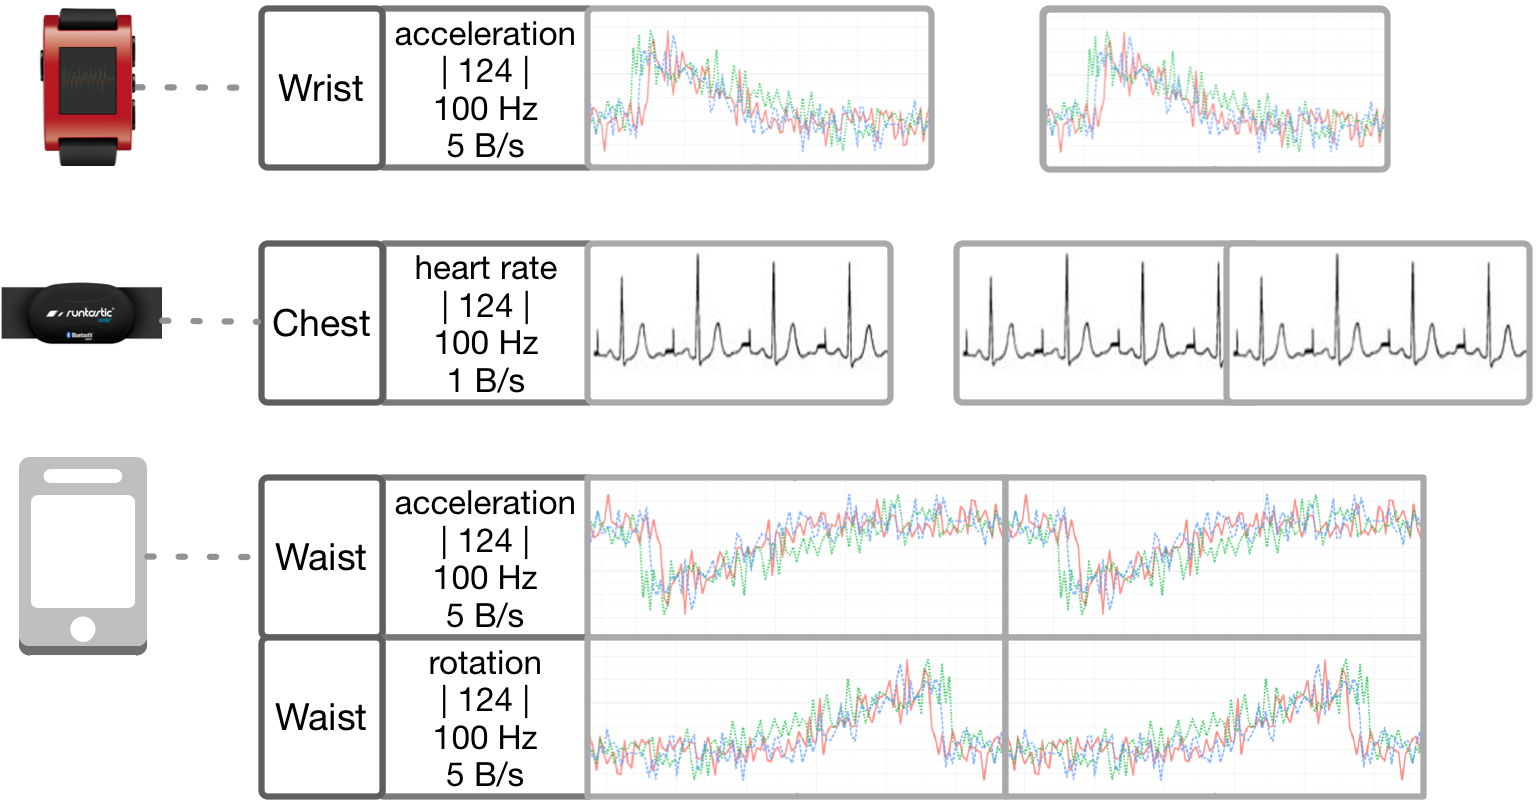
\includegraphics[width=7cm,keepaspectratio]{ri-sensor-fusion.png}
	\end{center}
\end{figure}

Once the sensor data from all sensors has been fused with respect to the sample time, the mobile application performs very simple signal processing: it smooths the signal by convolving it with a $3 \times 3$ kernel (\autoref{eq:smooth-kernel}).

\begin{equation} \label{eq:smooth-kernel}
	\begin{pmatrix}
	  ^1/_{16} & ^1/_8 & ^1/_{16} \\
	  ^1/_8    & ^1/_4 & ^1/_8    \\
	  ^1/_{16} & ^1/_8 & ^1/_{16}
	\end{pmatrix}
\end{equation}

Finally, the sensor data in the mobile application is a set of vectors containing 1 second of sensor input data, normalised to a range of $\interval[open]{-1}{1}$ by using a maximum reasonable value for acceleration, rotation, strain and heart rate. The maximum values are determined by the limitations of the sensor hardware together with reasonable limitations of human movement and together with the ranges of the protocol. For the three-value protocol used for the accelerometer and gyroscope data, and for the strain sensors, the limit of each element is the range of signed \SI{13}{\bit} integer: $\interval[open]{-4096}{4095}$. The unit of the measurement depends on the underlying sensor type: $0.01\ ms^{-2}$ for accelerometer, \SI{\pi/1800}{\radian\per\second} for gyroscope, TODO.

The fused and normalised sensor data is then passed as a single vector to the inputs of a muti-layer perceptron. The architecture of the MLP is driven by the sensor data as its inputs; for example, accelerometer-only MLP has 150 inputs (50 samples of the acceleration vector), the subsequent layer has 45 rectifier units, then 40 rectifier units, ending up with 32 softmax units, where 32 is the number of recognised setup movements. The architecture of the MLP for a fully-wired human has 1200 inputs, 250 rectifier units, 100 rectifier units, ending up with 32 softmax units. It is important to measure and optimise the power requirements for the computation; on iOS, we took advantage of the vDSP and veclib frameworks, which offer optimised vector operations. The MLP classes are not the exercises themselves, but the setup movements; one setup movement can map to multiple exercises. To provide accurate prediction of the exercise about to be started, the mobile application takes into account the expected exercise (given the user's typical behaviour), and the fine-grained location data. The information available in this context

\begin{table}[h]
\caption{Evaluation of a CNN for exercise vs. non-exercise classification}
\label{exercise}
\begin{center}
\begin{tabular}{|c||c||c|}
\hline
Actual / Predicted & Exercise & Non-exercise\\
\hline
Exercise & 12330 & 2305\\
\hline
Non-exercise & 3542 & 13412\\
\hline
\end{tabular}
\end{center}
\end{table}
